\section{Automatic Subtitles Positioning in 360-Video}

The recent popularization of omnidirectional cameras and Head-Mounted-Displays (HMDs) has increased the amount of 360-video content available \cite{mendes2020authoring}. These videos are spherical visual signals that allow the viewer to look around a full 360-degree view of a scene from a specific point. When using HMDs, at each instant in time, the viewer is presented with a viewport that is updated as the viewer moves their head. This type of content, especially when consumed through Virtual Reality~(VR) devices (HMDs included), can provide immersive experiences in which the user has a strong feeling of presence when compared with the use of traditional media \cite{montagud_culture_2020}. Due to this increasing popularity, we decided to investigate the usage of spatiotemporal localization of actors in 360-video.

Nowadays, the most common way for representing and transmitting 360-video is using an equirectangular projection~\cite{yang2018object}. With the equirectangular projection, each sphere point is defined by two angles~\cite{snyder1987map}: \emph{latitude}~$\theta \in [-90^{\circ}, +90^{\circ}]$ and \emph{longitude}~$\phi \in [-180^{\circ}, +180^{\circ}]$. This kind of projection creates challenges for image processing and computer vision algorithms, especially to the convolution-based ones because of the severe distortions in areas vertically distant from the center of the image~(see Figure \ref{fig:equirectangular_proj}).

\begin{figure}[!ht]
\centering
    \begin{subfigure}{0.47\linewidth}
        \centering
        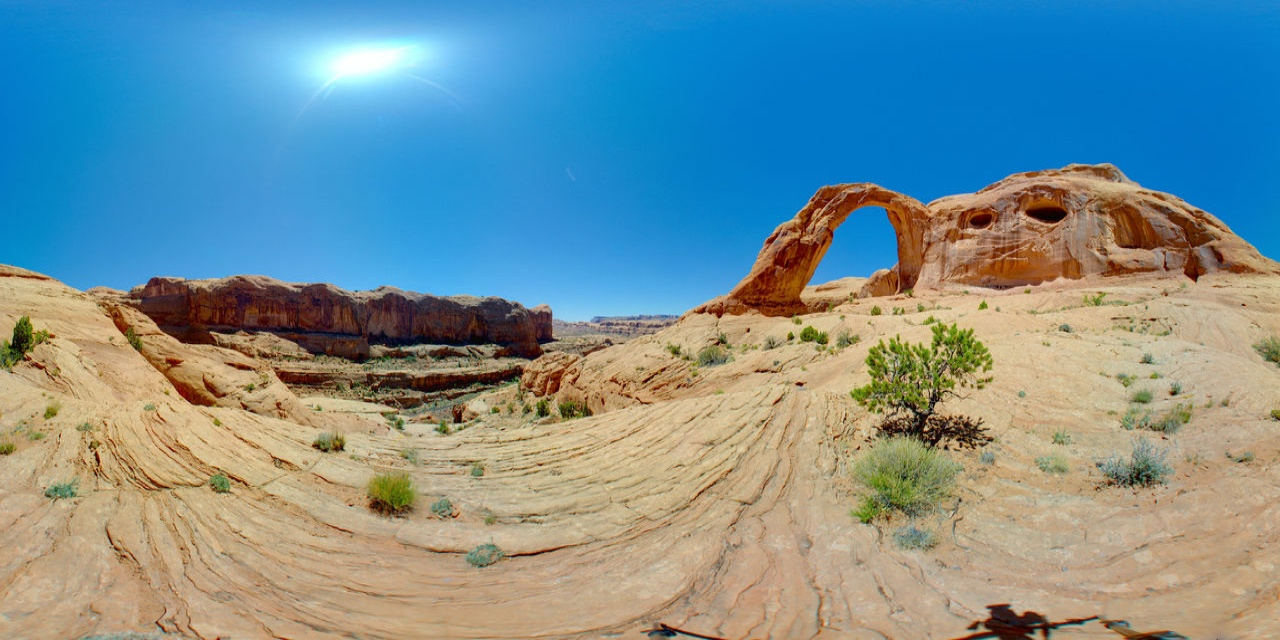
\includegraphics[width=1\textwidth]{img/image (9).jpg}
        \caption{Outdoor equirectangular image.}
        \label{subfig:out_equi}
    \end{subfigure}\hfill
    \begin{subfigure}{0.47\linewidth}
        \centering
        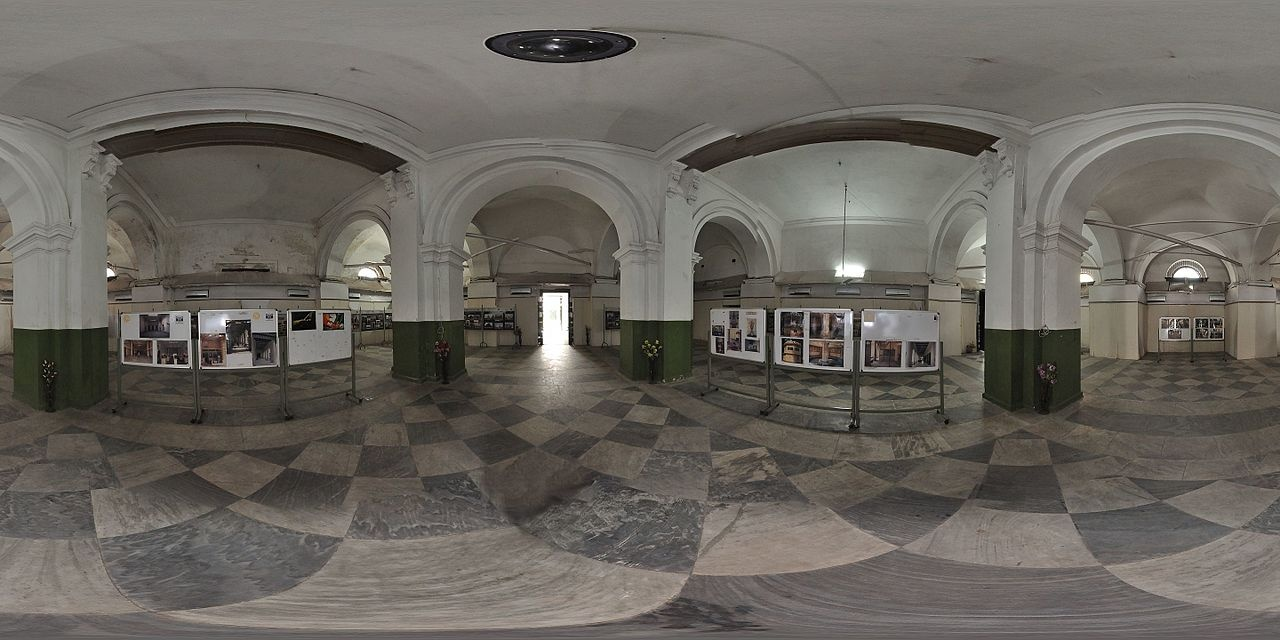
\includegraphics[width=1\textwidth]{img/image (10).JPG}
        \caption{Indoor equirectangular image.}
        \label{subfig:in_equi}
    \end{subfigure}

\caption{Examples of 360-images represented through equirectangular projection.}
\label{fig:equirectangular_proj}
\end{figure}

Due to these distortions, we adapted the steps of our methods that use traditional CNNs: \emph{Face Detection} and \emph{Embeddings Generation}. These adaptations are described in Sections \ref{subsec:360_adaptations}. In Section \ref{subsec:dynamic_subtitles}, we describe how these adaptations can be used for subtitles positioning in 360-videos.

\subsection{Face Detection and Embeddings Generation in 360-Videos}
\label{subsec:360_adaptations}

Because of the distortions present on the equirectangular projection, we opted for elaborating a solution based on viewports extraction. A viewport is defined by its center, in polar coordinates~(lat, long), and its field of view~(FoV). Figure \ref{fig:viewports} shows viewports extracted at different polar coordinates from Figure \ref{subfig:out_equi}.

\begin{figure}[!ht]
    \centering
    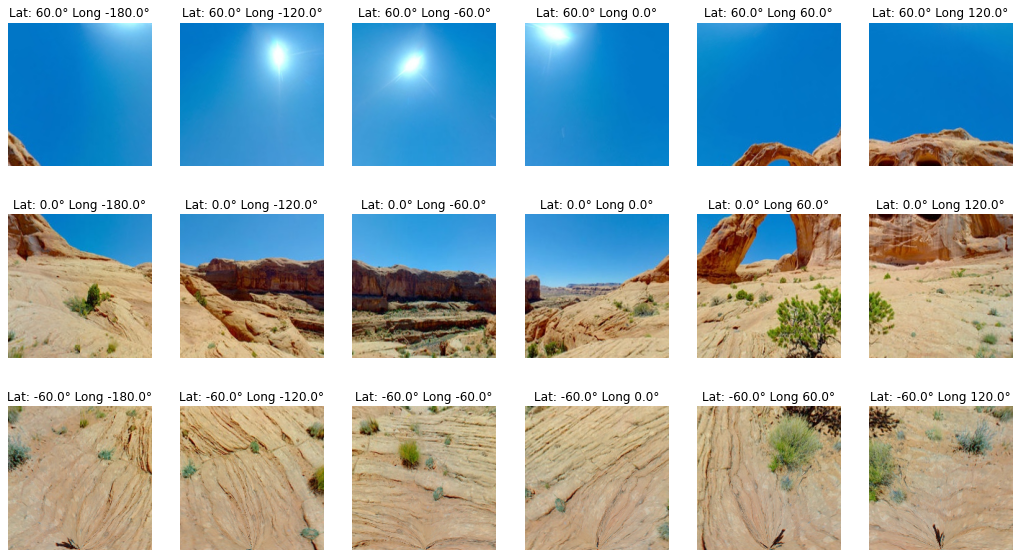
\includegraphics[width=1\textwidth]{img/viewports.png}
    \caption{Viewports extracted at different polar coordinates with $FoV = 60^{\circ}$}
    \label{fig:viewports}
\end{figure}

For each viewport, we apply a face detection model. 
Then, we project the faces detected bounding boxes back to the equirectangular image. For doing that for a given bounding box, we project the four corners and the mean point of each edge~(8 points in total). Therefore, in the equirectangular image, we deal with polygons instead of bounding boxes, due to the distortions introduced. As different viewports may intersect and cover part of the same region in an image, we apply Non-maximum Supression~(NMS), eliminating intersected detections within a given threshold. One of the main advantages of this approach is that we can use face detection models trained in regular images, since distortions are reduced with the use of viewports. In order to test this approach, we have created a synthetic dataset.

Due to the lack of datasets for face detection in equirectangular images, we created a synthetic dataset based on the FDDB dataset~\cite{fddbTech}, a popular benchmark for face detection evaluation containing 2845 images and 5171 faces. We collected 19 indoor and outdoor equirectangular images, from Google Images,\footnote{https://www.google.com/imghp} ESO,\footnote{https://www.eso.org/public} and PxHere.\footnote{https://pxhere.com}
For each image in the FDDB dataset, we randomly chose a latitude, longitude and equirectangular image to project it. For each face present on that image, we projected the bounding box to a polygon exactly as mentioned in the viewport process. Figure \ref{fig:fddb_proj} shows an example of an image from FDDB projected in the polar coordinates \emph{lat} $ = -60^{\circ}$ \emph{long} $= 0^{\circ}$ to an equirectangular image.

\begin{figure}[!ht]
\centering
    \begin{subfigure}{0.4\linewidth}
        \centering
        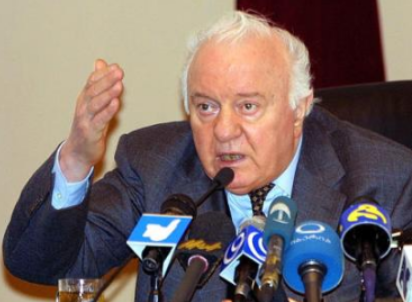
\includegraphics[height=10em]{img/face_pre.png}
        \caption{FDDB image example.}
        \label{subfig:face_pre}
    \end{subfigure}\hfill
    \begin{subfigure}{0.55\linewidth}
        \centering
        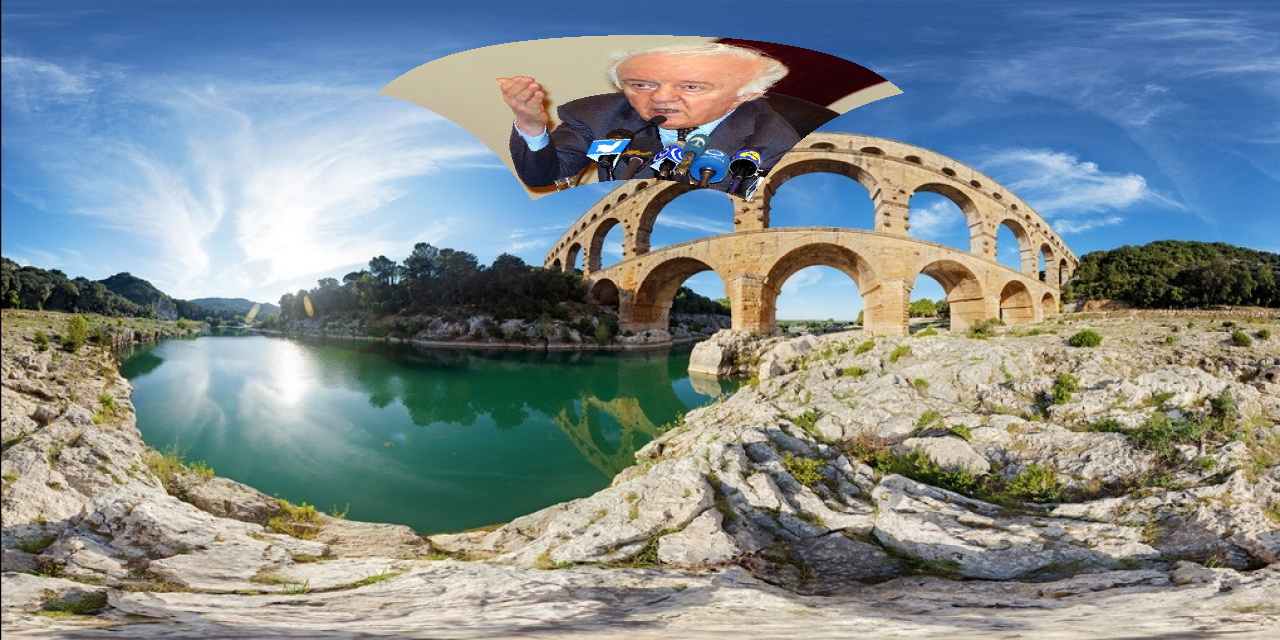
\includegraphics[height=10em]{img/face_pos.png}
        \caption{Projection example of FDDB image.}
        \label{subfig:face_pos}
    \end{subfigure}

\caption{FDDB image projection to Equirectangular image.}
\label{fig:fddb_proj}
\end{figure}

After eliminating repeated detections with NMS, we perform \emph{Embeddings Generation} using the faces detected in the viewports~(with reduced distortions) instead of using its equivalent in the original equirectangular video frame.

For this part of our work, we have defined the following remaining task.

\begin{itemize}
    \item \textbf{T 1}: Model test using MTCNN and MTCNN with viewports~(80\% complete).
\end{itemize}

\subsection{Authoring Model for Interactive 360-Videos}
\label{subsec:dynamic_subtitles}

In \cite{mendes2020authoring}, we proposed a model for authoring interactive 360° video. In such a model, we can define interactive 360° video that are presented together with additional information attached to it, such as image, text and spatial audio. The positioning of such additional information is defined by their polar coordinates, start time and duration. Moreover, we can also configure behaviours depending on where the user is looking. For instance, we can define that a text moves with the user's head motion and is always visible or that such text is placed at fixed position if it is in the field of view of the user. Besides the design of such a model, we developed a player that follows the definitions of our model and is able to play interactive 360° video defined by it. Then, we can use the results obtained from the previous phase to define the positioning of subtitles according to the actors positioning using our player.